Now lets consider how the charging and discharging of the receiver circuit works. According to manufacturer specification $i_r \leq 400 $ mA , which enforces the limit for the system to function properly.
In figure %~\ref{fig:rec_design}
the super capacitor $C_s$ has very low series resistance of $0.07 \Omega$ compared to $R_L = 65 \Omega$ hence during charging we can say that $i_c \approx i_r$ and if the $i_r(t)$ is not constant and depends on time then the capacitor charging is governed by the following equation
\begin{equation}\label{eq:cap}
 V_c = V_{reg} \left(1 - e^{\frac{-t}{R_cC}}\right)
\end{equation}
where $R_c$ is the series limiting resistance of receiver circuit whose value depends on the maximum value of $i_r$ and $C$ is the total capacitance of super capacitor which in our case $C_s = 5 $ Farads
$R_c$ can be chosen using $R_c = \frac { V_{reg}}{i_r} $ for maximum allowed $i_r = 400$ mA which gives us $R_c = 12.5 \Omega$

\begin{figure}[h!]
\centering
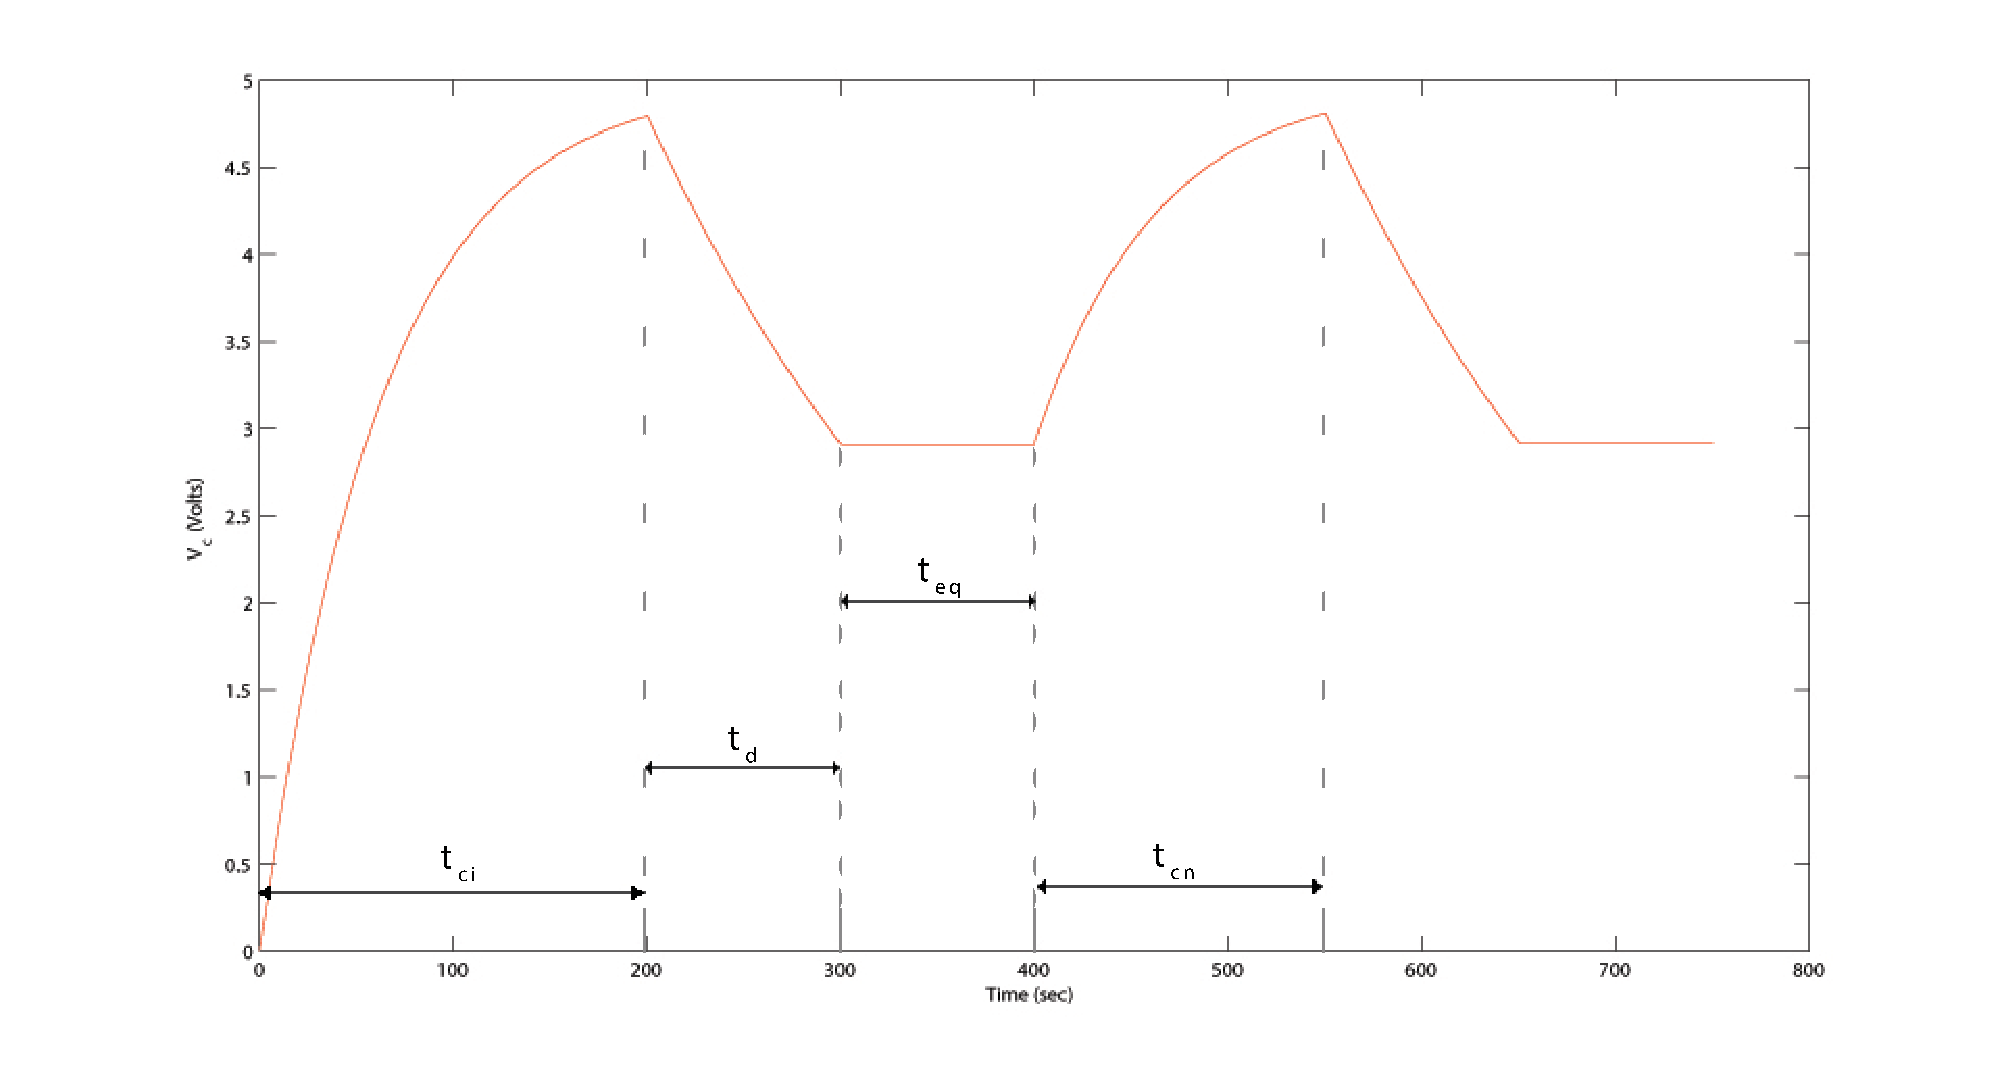
\includegraphics[width=1\textwidth]{cd_cycle.pdf}
\caption{Charging profile of the super capacitor }
\label{fig:ch_profile}
\end{figure}

Figure \ref{fig:ch_profile} shows charging, discharging and idle profile of the super capacitor during the system operation. In initial charging cycle $t_{ci}$, $C_s$ is charged using $i_r(t)$ following equation \ref{eq:cap} and during discharge cycle $t_d$, the $i_r(t) = 0$ and discharge current is supplied in the form of $i_b$ and $i_L$. Finally during the equilibrium cycle $t_{eq}$ the voltage is reduced to equal the battery voltage ($V_l = 3$ V) such that no current flows between the battery and super capacitor and $i_b = 0$, at this stage only battery's charge is used to power the LED. At last during the second charge cycle $t_{c2}$, the capacitor's charging starts from equilibrium voltage instead of 0 and is charged to $V_{reg}$ un till the discharge cycle starts again.
